\documentclass[border=10pt]{standalone}
\usepackage[T1]{fontenc}
\usepackage{amsmath}
\usepackage{tikz}
\usepackage[svgnames]{xcolor}
\usetikzlibrary{shapes.geometric, arrows.meta, positioning, calc, fit,
                 decorations.pathreplacing}

% ---------------------------------------------------------------
% Colour palette (matches solver_flowchart.tex)
% ---------------------------------------------------------------
\colorlet{OrangeFill}{LightSalmon}
\colorlet{OrangeLine}{DarkSalmon!30!Chocolate}
\colorlet{GreenFill}{MediumAquamarine}
\colorlet{GreenLine}{MediumAquamarine!30!Teal}
\colorlet{PurpleFill}{MediumPurple}
\colorlet{PurpleLine}{MediumPurple!30!SlateBlue}
\colorlet{PinkFill}{Thistle}
\colorlet{PinkLine}{Thistle!30!Plum}
\colorlet{BlueFill}{LightSkyBlue}
\colorlet{BlueLine}{SteelBlue}
\colorlet{GrayFill}{LightGray!60!OldLace}
\colorlet{GrayLine}{RosyBrown!50!Silver}

\begin{document}
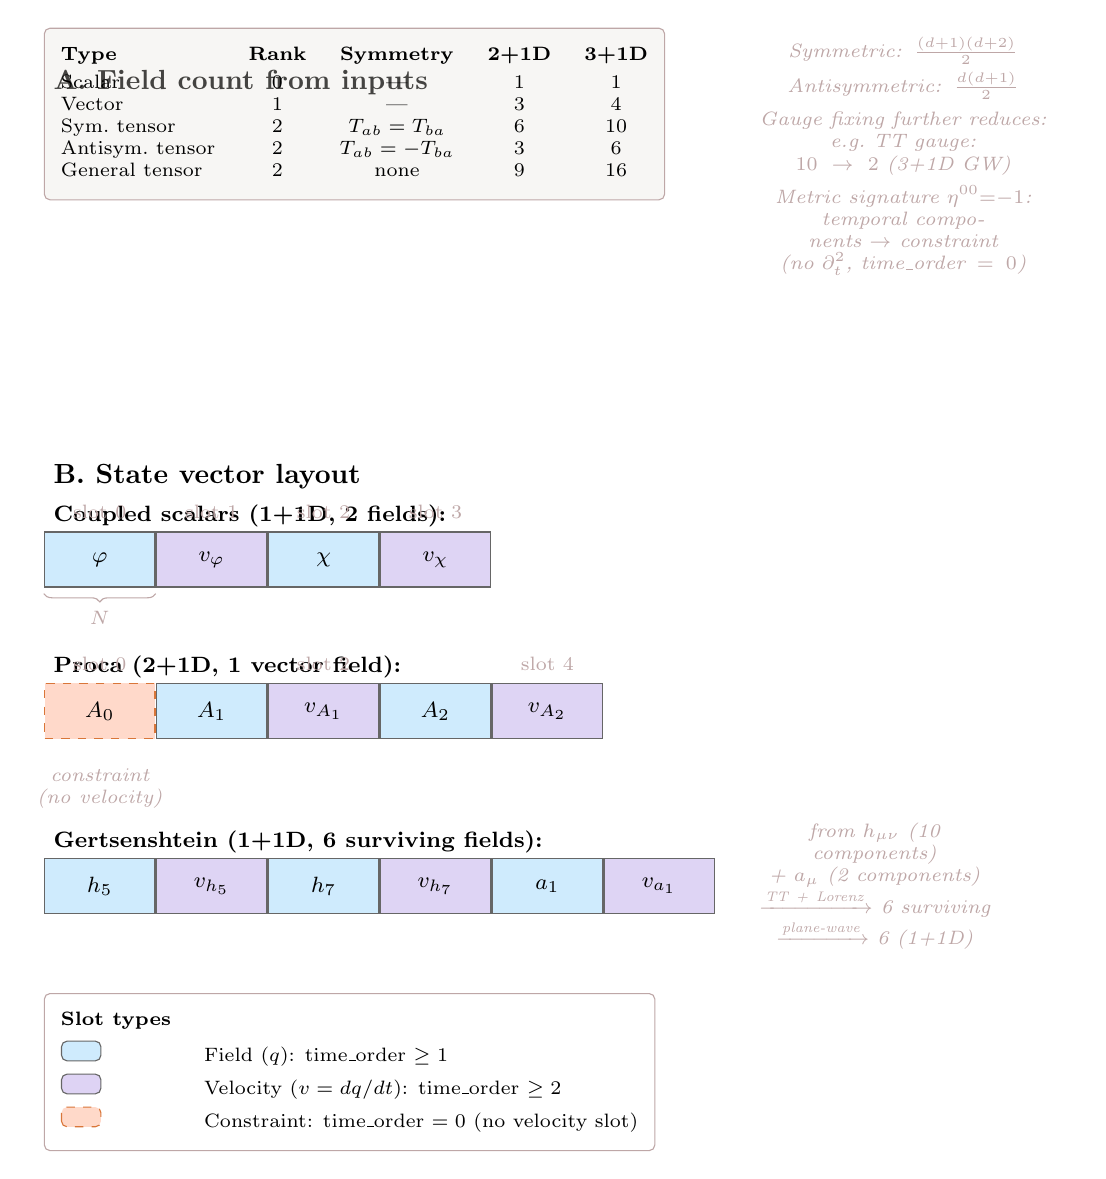
\begin{tikzpicture}[
    slot/.style={
        rectangle, minimum width=1.4cm, minimum height=0.7cm,
        draw=black!60, line width=0.6pt, font=\footnotesize,
        align=center, text opacity=1, text=black
    },
    fieldslot/.style={slot, fill=BlueFill, fill opacity=0.4},
    velslot/.style={slot, fill=PurpleFill, fill opacity=0.3},
    conslot/.style={slot, fill=OrangeFill, fill opacity=0.4, draw=OrangeLine, dashed},
    lbl/.style={font=\footnotesize\bfseries, text=black},
    annot/.style={font=\scriptsize\itshape, text=GrayLine, align=center},
    arr/.style={-{Stealth[length=4pt, width=3pt]}, semithick, black!70},
    node distance=0cm
]

% ===================================================================
% PART A: Field generation from inputs (top)
% ===================================================================
\node[font=\normalsize\bfseries, anchor=west] (titleA) at (0, 0)
    {A. Field count from inputs};

\node[below=0.4cm of titleA.west, anchor=west,
      rectangle, rounded corners=2pt, draw=GrayLine,
      fill=GrayFill, fill opacity=0.3, inner sep=6pt,
      font=\scriptsize, align=left, text opacity=1] (table) {%
\begin{tabular}{@{}l c c c c@{}}
    \textbf{Type} & \textbf{Rank} & \textbf{Symmetry}
    & \textbf{2+1D} & \textbf{3+1D} \\[2pt]
    Scalar & 0 & --- & 1 & 1 \\
    Vector & 1 & --- & 3 & 4 \\
    Sym.\ tensor & 2 & $T_{ab}=T_{ba}$ & 6 & 10 \\
    Antisym.\ tensor & 2 & $T_{ab}=-T_{ba}$ & 3 & 6 \\
    General tensor & 2 & none & 9 & 16 \\
\end{tabular}};

% Formula annotation
\node[annot, right=0.8cm of table.north east, anchor=north west,
      text width=4.2cm] (formula) {%
    Symmetric: $\frac{(d{+}1)(d{+}2)}{2}$\\[2pt]
    Antisymmetric: $\frac{d(d{+}1)}{2}$\\[4pt]
    Gauge fixing further reduces:\\
    e.g.\ TT gauge: $10 \to 2$ (3+1D GW)\\[4pt]
    Metric signature $\eta^{00}{=}{-}1$:\\
    temporal components $\to$ constraint\\
    (no $\partial^2_t$, time\_order${}=0$)};

% ===================================================================
% PART B: State vector examples (bottom)
% ===================================================================
\node[font=\normalsize\bfseries, anchor=west] (titleB)
    at (0, -5.0) {B. State vector layout};

% --- Example 1: Coupled scalars ---
\node[lbl, below=0.5cm of titleB.west, anchor=west] (ex1lbl)
    {Coupled scalars (1+1D, 2 fields):};

\node[fieldslot, below=0.2cm of ex1lbl.west, anchor=north west] (s1a) {$\varphi$};
\node[velslot, right=of s1a] (s1b) {$v_\varphi$};
\node[fieldslot, right=of s1b] (s1c) {$\chi$};
\node[velslot, right=of s1c] (s1d) {$v_\chi$};

% N annotation
\draw[decorate, decoration={brace, amplitude=3pt, mirror, raise=2pt},
      GrayLine]
    (s1a.south west) -- (s1a.south east)
    node[midway, below=5pt, font=\scriptsize, text=GrayLine] {$N$};

% Slot indices
\node[font=\scriptsize, text=GrayLine, above=1pt of s1a] {slot 0};
\node[font=\scriptsize, text=GrayLine, above=1pt of s1b] {slot 1};
\node[font=\scriptsize, text=GrayLine, above=1pt of s1c] {slot 2};
\node[font=\scriptsize, text=GrayLine, above=1pt of s1d] {slot 3};

% --- Example 2: Proca 2+1D ---
\node[lbl, below=1.0cm of s1a.south west, anchor=west] (ex2lbl)
    {Proca (2+1D, 1 vector field):};

\node[conslot, below=0.2cm of ex2lbl.west, anchor=north west] (s2a) {$A_0$};
\node[fieldslot, right=of s2a] (s2b) {$A_1$};
\node[velslot, right=of s2b] (s2c) {$v_{A_1}$};
\node[fieldslot, right=of s2c] (s2d) {$A_2$};
\node[velslot, right=of s2d] (s2e) {$v_{A_2}$};

% Constraint annotation
\node[annot, below=0.25cm of s2a] {constraint\\(no velocity)};

\node[font=\scriptsize, text=GrayLine, above=1pt of s2a] {slot 0};
\node[font=\scriptsize, text=GrayLine, above=1pt of s2c] {slot 2};
\node[font=\scriptsize, text=GrayLine, above=1pt of s2e] {slot 4};

% --- Example 3: Gertsenshtein 1+1D ---
\node[lbl, below=1.3cm of s2a.south west, anchor=west] (ex3lbl)
    {Gertsenshtein (1+1D, 6 surviving fields):};

\node[fieldslot, below=0.2cm of ex3lbl.west, anchor=north west] (s3a) {$h_5$};
\node[velslot, right=of s3a] (s3b) {$v_{h_5}$};
\node[fieldslot, right=of s3b] (s3c) {$h_7$};
\node[velslot, right=of s3c] (s3d) {$v_{h_7}$};
\node[fieldslot, right=of s3d] (s3e) {$a_1$};
\node[velslot, right=of s3e] (s3f) {$v_{a_1}$};

\node[annot, right=0.4cm of s3f.east, anchor=west, text width=3.0cm]
    {from $h_{\mu\nu}$ (10 components)\\
     + $a_\mu$ (2 components)\\
     $\xrightarrow{\text{TT + Lorenz}}$ 6 surviving\\
     $\xrightarrow{\text{plane-wave}}$ 6 (1+1D)};

% ===================================================================
% LEGEND
% ===================================================================
\node[below=1.0cm of s3a.south west, anchor=north west,
      draw=GrayLine, rounded corners=2pt, inner sep=6pt,
      fill=white, font=\scriptsize] (legend) {%
\begin{tabular}{@{}l l@{}}
    \textbf{Slot types} \\[3pt]
    \tikz\fill[BlueFill, fill opacity=0.4, draw=black!60]
        (0,0) rectangle (0.5,0.25); & Field ($q$): time\_order $\geq 1$ \\[2pt]
    \tikz\fill[PurpleFill, fill opacity=0.3, draw=black!60]
        (0,0) rectangle (0.5,0.25); & Velocity ($v = dq/dt$): time\_order $\geq 2$ \\[2pt]
    \tikz\fill[OrangeFill, fill opacity=0.4, draw=OrangeLine, dashed]
        (0,0) rectangle (0.5,0.25); & Constraint: time\_order $= 0$ (no velocity slot) \\
\end{tabular}};

\end{tikzpicture}
\end{document}
